\chapter{}

\begin{figure}
\centering
\includegraphics[width=0.6\linewidth]{30/as-vésperas.png}
\caption{Às vésperas de deixar Araraquara.}
\end{figure}

Em janeiro de 1982, passado o período das festas de fim de ano, deixamos Araraquara.
Eu estava entre aliviada e apreensiva.
Aliviada, por me distanciar daquela terra e daquela situação que se criara com a morte do meu pai, mas, principalmente, porque longe daquilo tudo nós estaríamos livres para construir nossa vida e educar nossos filhos segundo nossos próprios valores.
Apreensiva, por não ter a menor ideia do que nos esperava naquele lugar remoto.
Paulo me levara algumas fotos e por elas dava para ver que a cidade era pobrezinha, embora tivesse três pequenos hospitais e uma Fundação Bradesco, uma escola-modelo mantida pelo banco com o objetivo prioritário de capacitar mão de obra para as agências espalhadas na região.
Afora isso, duas ruas asfaltadas e energia elétrica garantida por geradores a diesel, desligados pontualmente às vinte e uma horas.

\begin{figure}
\hfill
\centering
\begin{subfigure}[h]{0.48\linewidth}
\centering
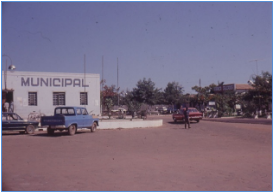
\includegraphics[width=\linewidth]{30/ca-1.png}
\end{subfigure}
\hfill
\begin{subfigure}[h]{0.48\linewidth}
\centering
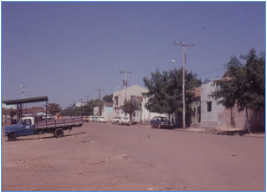
\includegraphics[width=1\linewidth]{30/ca-2.png}
\end{subfigure}
\caption{Conceição do Araguaia, Pará, em 1982}
\end{figure}

A viagem foi cheia de novidades para as crianças e para mim.
A bordo da nossa perua Ford Belina conhecemos a mítica Belém-Brasília que trilhamos do início até Guaraí.
Um colchão arrumado no porta-malas acomodava os pequenos, enquanto os maiores dividiam o banco traseiro.
Um caminhão seguia com a mudança.
Em Guaraí, enveredamos em direção ao Pará por uma estrada de terra que nos levou aos solavancos até Conceição e, de lá, à Fazenda Nazaré do Araguaia, uma das propriedades do grupo, onde nos hospedaríamos até conseguir uma casa na cidade.

Chegamos à tardezinha e me impressionou o ar de abandono de tudo, o mato alto, os pastos maltratados.
Entretanto, as construções pareciam boas e a casa-sede era muito bonita.
Instalada numa elevação que permitia enxergar boa parte da fazenda, imitava um rancho californiano, com as duas alas de quarto dispostas em torno de um pátio interno e a fachada imponente onde se destacava a larga varanda sustentada por robustos pilares de pau-brasil.

Esperava-nos o advogado e sócio minoritário dos irmãos Gomes dos Reis, um tal Doutor James.
De uma gentileza melíflua, apresentou-nos a casa, indicou-nos os quartos e recomendou-nos à caseira, uma nordestina alta e magra, cara de poucos amigos.
Assim que acomodamos nossas bagagens, fomos convidados à sala onde nos esperava um aperitivo, seguido do jantar.
Alguma coisa naquele almofadinha de sapatos polidos pôs em guarda a filha de Mathias Filpi.
Mas, cansados como estávamos, deixei para pensar nisso depois.
Tratei de pôr as crianças na cama e Paulo ficou lá, conversando com a escorregadia figura.
De madrugada, tive a confirmação dos meus presságios: ouvindo um leve ruído na porta da frente, espiei pelas largas venezianas da janela e vi a criatura, sorrateira, erguendo os pontudos joelhos para não roçar a barra das calças e os sapatos brilhantes no mato encharcado de orvalho, erguer a pasta de documentos sobre a cabeça e atravessar, pé ante pé, o pátio fronteiro à casa e lá embaixo, diante da casa do capataz, embarcar numa caminhonete e desaparecer na curva da estrada.
 

Ao amanhecer, comuniquei ao Paulo a inopinada partida do nosso anfitrião e, já esperando pelo pior, fui até a cozinha ver como andavam os preparativos para o café.
Dito e feito: sobre a mesa da sala ainda se espalhavam os restos do jantar e, na cozinha, o fogão apagado e a desordem da véspera indicavam que eu teria problemas com a nossa caseira.
Em pouco tempo nos inteiraríamos da situação: a fazenda estava entregue há muito tempo a um capataz cearense que lá se arranchara com parentes e aderentes e o bando, beneficiado pela permanente ausência dos patrões, vivia na mais completa vadiagem, sustentado pela venda semanal, nos açougues da cidade, das reses subtraídas ao rebanho de milhares de nelores puríssimos que deveriam estar povoando aqueles pastos transformados em quiçaça.

Sentindo o sangue subir à cabeça, invadi a casa dos folgados e me deparei com uma cena idílica: às nove da manhã, refestelado na rede, o tal administrador entregava-se aos cafunés da caseira, sua mulher.
Não dei tempo para que se recuperassem do susto e ordenei que ela fosse imediatamente para o serviço ou juntasse os trens e se pusesse na estrada.
E revelei o que eles pareciam ignorar: Paulo estava ali com autoridade sobre aquela e todas as outras fazendas do grupo e que a boa-vida tinha acabado.
Minha raiva não permitiu consultar meu marido sobre a veracidade ou a oportunidade daquele comunicado.
Que se danasse! Eu não estava com a mínima vontade de me controlar.
Alguma coisa me dizia que teríamos mais algumas más surpresas pela frente.

Em poucos dias ficou evidente que os cearenses não se enquadrariam mesmo e Paulo teve que despedi-los.
Nas outras fazendas, a situação não diferia muito.
Porém, eu tinha outras coisas com que me preocupar: o período de aulas começaria em breve e nós tínhamos que achar uma casa na cidadezinha.
Tomaz, Marcelo e Fernando foram matriculados na Fundação Bradesco, único estabelecimento que funcionava regularmente na região.
A educação pública no estado do Pará era mais do que precária, era imoral.
Só para dar uma ideia, o único colégio do lugar, grande por sinal, com cerca de três mil alunos matriculados, durante o tempo em que moramos lá, não conseguiu uma única vez cumprir o ano letivo como estabelecido por lei, seja por falta de professores ou de material para manter as salas funcionando.
Por dois anos sucessivos, um providencial incêndio na secretaria da escola incinerou todos os registros e, no ano seguinte, e de novo no outro, os alunos tiveram que repetir a série que, supostamente, tinham acabado de cursar.

Paula, que ainda estava na pré-escola, frequentaria ``O Sossego da Mamãe'', uma escolinha maternal mantida por duas professoras mineiras.
Vicente ficaria em casa por mais um ano.

Depois de muito percorrermos as arenosas ruas de Conceição em busca de uma casa para alugar, um noivado desmanchado às vésperas do casamento foi a nossa salvação.
A casa, novinha em folha, nos foi oferecida pelo jovem noivo que, diga-se de passagem, não parecia muito frustrado com a mudança de planos.
O grande atrativo da moradia e que motivou um aluguel elevado para os padrões do lugar era a suíte do casal, cujo banheiro ostentava uma pia de acrílico, objeto de romaria por parte dos parentes e conhecidos do rapaz durante ainda umas duas semanas depois que nos mudamos.

\begin{figure}
\centering
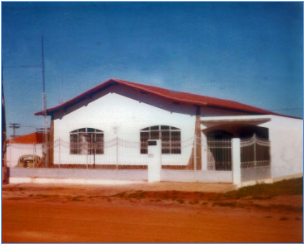
\includegraphics[width=0.8\linewidth]{30/nossa-casa.png}
\caption{Nossa casa em Conceição.}
\end{figure}

\begin{figure}
\centering
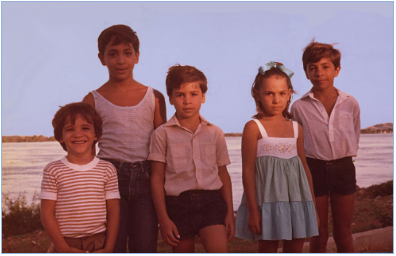
\includegraphics[width=0.8\linewidth]{30/beira-do-araguaia.png}
\caption{À beira do rio Araguaia.}
\end{figure}

\begin{figure}
\centering
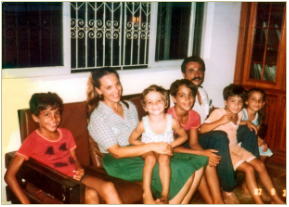
\includegraphics[width=0.8\linewidth]{30/prontos-para-durmir.png}
\caption{Prontos para dormir, na nova casa.}
\end{figure}

\begin{figure}
\centering
\includegraphics[width=0.8\linewidth]{30/recomeçando.png}
\caption{Recomeçando a vida em Conceição.}
\end{figure}

A minha adaptação à vida de Conceição não foi fácil.
Diferentemente da experiência na Bodoquena, agora eu tinha cinco filhos e o futuro deles me preocupava dia e noite.
Será que tínhamos o direito de privá-los de uma aprendizagem de melhor qualidade, como aquela que as primas tinham no rico estado de São Paulo?  

Cerca de três meses depois da nossa chegada, o salário do Paulo começou a atrasar e, logo em seguida, deixou de ser depositado.
Os telefonemas não tinham retorno e o desespero bateu.

Durante os anos setenta, oitenta, organismos como SUDAM (Superintendência do Desenvolvimento da Amazônia) e SUDENE (Superintendência do Desenvolvimento do Nordeste), pretensamente criados com o objetivo de incentivar a ocupação e o desenvolvimento de regiões atrasadas ou inexploradas do país, por meio de incentivos fiscais e generosa oferta de financiamentos, viraram um manancial de dinheiro a fundo perdido para muitos empresários do sul e sudeste, e um excelente meio para dar vazão aos chamados ``caixa-dois''.
Houve, é claro, quem utilizasse seriamente os financiamentos obtidos por esta via, mas esse não parecia ser o caso da Nazaré, do Curral de Pedra e das demais fazendas dos Gomes dos Reis.
Esses irmãos eram empresários respeitáveis de Jaú, donos de fazenda considerada modelo de gestão por muitos anos naquela região, mas eram agora bastante idosos e começavam a delegar aos herdeiros a missão de levar adiante os negócios.
E a partir daí é que tudo começou a desandar, como estávamos percebendo.

O dinheiro em casa escasseou e o arrependimento ameaçou tomar conta de mim.
Mas, por mais que eu buscasse uma saída, não tinha volta possível na decisão que eu tomara.
No final da tarde, após terminar a sessão das tarefas, eu costumava levar os meninos ao clube, designação eufêmica para uma piscina construída no alto de uma colina, a cavaleiro do rio, aonde se chegava contornando o bordel da cidade.
Ao fundo, uma cobertura de palha abrigava um freezer fechado a cadeado.
Havia um projeto de construção, pelo que se depreendia a partir dos vestígios de alicerces que apontavam no meio do capim crescido, porém estava-se ali diante de um impasse: os associados não pagavam a mensalidade porque não havia clube e não havia clube porque os sócios não pagavam a mensalidade, como me explicou o diretor.
Sentada no chão, à beira da piscina, enquanto as crianças brincavam, eu chorava e me consolava com a visão do imenso Araguaia dourado pelo sol poente.


Paulo começou a se virar para todos os lados.
Caíramos num engodo, eu não tinha mais dúvidas.
A esperança é que o financiamento da seringueira saindo, pelo menos os atrasados nos fossem pagos.
De grande valia para nós foi a amizade do Zezão, um comerciante de produtos agropecuários com loja em Conceição e em outras cidades próximas e muito conhecido entre os fazendeiros do lugar.
Ele começou a divulgar a notícia de que Paulo era especialista em cultivo de seringueira e logo começaram a aparecer interessados em adquirir mudas, encomendar projetos de financiamento e obter assistência técnica.
Foi assim que começamos a respirar novamente.
O contrato com os Gomes dos Reis passou por alteração e o pagamento do Paulo ficou melhor amarrado no projeto deles para o financiamento das seringueiras, em processo de aprovação na SUDAM.